\subsection{Serviço de Backups}

O servidor de \emph{Backups} utilizado neste caso é o Servidor \emph{Arkeia}.

O \emph{Arkeia} é uma excelente solução para a salvaguarda de dados sendo um auxiliar importante em acções de \emph{disaster recovery}. O \emph{Arkeia} oferece uma resposta cabal em termos de desempenho, flexibilidade e confiabilidade para todo o tipo e volume dados a salvaguardar.

O \emph{Arkeia} é rápido, fácil de usar, sendo compatível com praticamente qualquer combinação de computadores, sistemas operativos e dispositivos de armazenamento. A salvaguarda de dados pode facilmente ser feita de forma global ou incremental preservando a estrutura de directorias, \emph{links} simbólicos e quaisquer atributos especiais do sistema de ficheiros.

Para determinadas plataformas existe a possibilidade de aquisição de \textit{plugins} para efectuar \textit{Hot Backups} de dados do Oracle, MySQL, etc.

Informações adicionais podem ser obtidas em:\\ \begin{normalsize}\sffamily\href{http://www.arkeia.com/products/arkeianetworkbackup/index.php}{www.arkeia.com/products/arkeianetworkbackup/index.php}\end{normalsize}

Os ficheiros de configuração deste serviço estão na localização por omissão. Para mais informações deverá consultar o manual do produto.


O conteúdo do servidor está localizado em:

\begin{Verbatim}
C:\Program Files\Arkeia
\end{Verbatim}

O comando para controlar este serviço (iniciar/parar) é o seguinte:

\begin{figure}[H]
    \begin{center}
        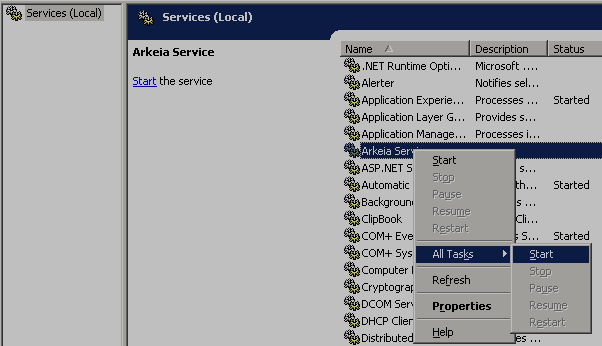
\includegraphics[width=10cm]{include/img/ark-win-start}
    \end{center}
    \caption{Iniciar o Arkeia}
    \label{fig:ARK-WIN1}
\end{figure}


\begin{figure}[H]
    \begin{center}
        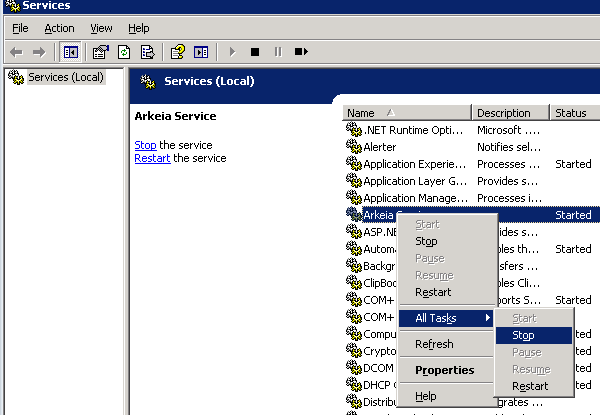
\includegraphics[width=10cm]{include/img/ark-win-stop}
    \end{center}
    \caption{Parar o Arkeia}
    \label{fig:ARK-WIN2}
\end{figure}



